\chapter{Results}

\indent This chapter presents the results of the measurements of the cross sections of the coherent $\pi^{0}$ photoproduction on $^{116}Sn$, $^{120}Sn$ and  $^{124}Sn$. The experimental data are compared with the theoretical DREN Kamalov's calculations.

\section{Cross sections}

\indent The three tin isotopes have been chosen for this experiment because they are all stable nuclei and because their proton number is a magic number. Also, investigating the nuclear matter structure along the isotopic chain offers an additional advantage that the data for each target can be compared with each other without a systematic error due to charge distribution, and therefore allows to accurately measure the changes in the nuclear structure predicted by different models. The details of the targets used in the study are summarized in the table \ref{table_targets}, in chapter 3.

\indent The differential cross sections for all the targets are presented in figures \ref{cross_section1} - \ref{cross_section3}. The diffraction pattern due to the form factor presence in the cross section is clearly visible.

\begin{figure}[H]
\begin{center}
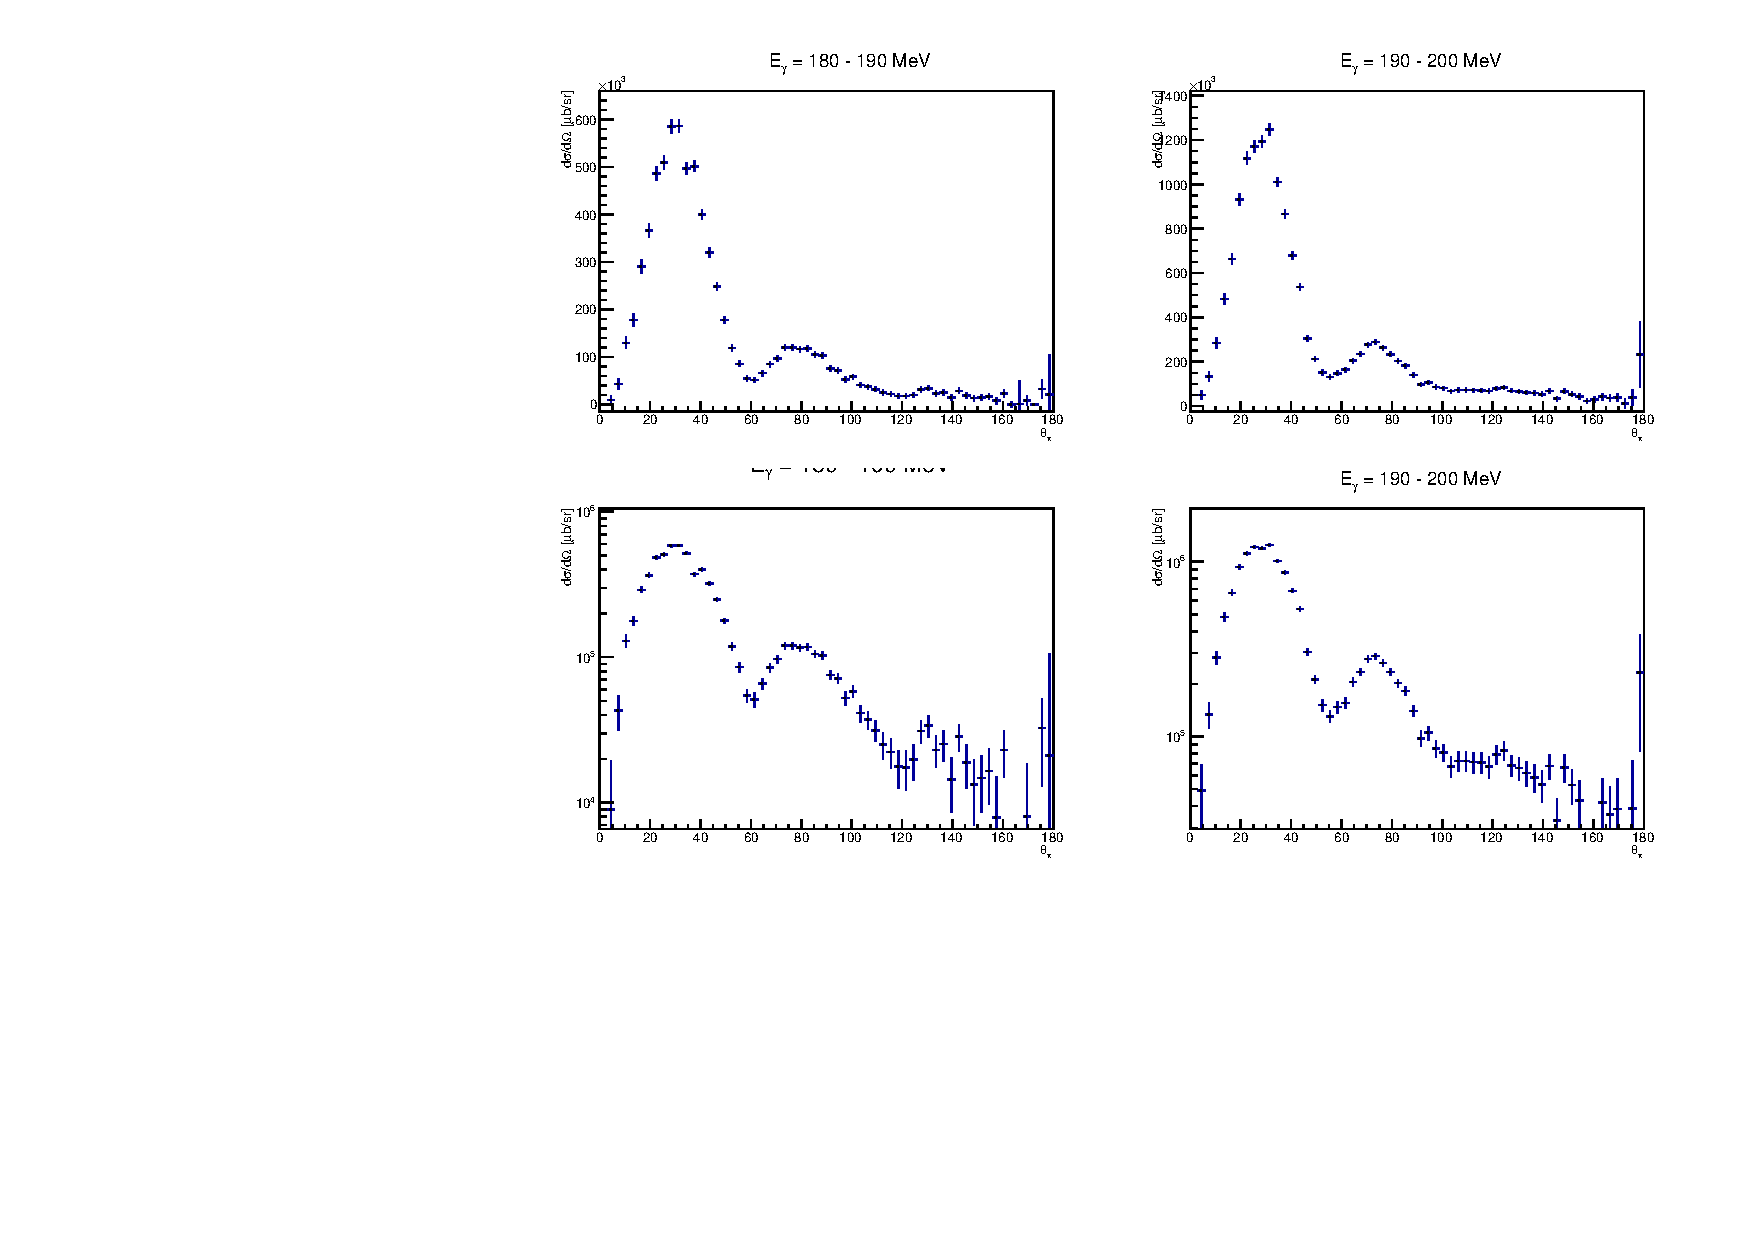
\includegraphics[scale=0.55]{pictures/pdf/sn116_cross_section_1.pdf}
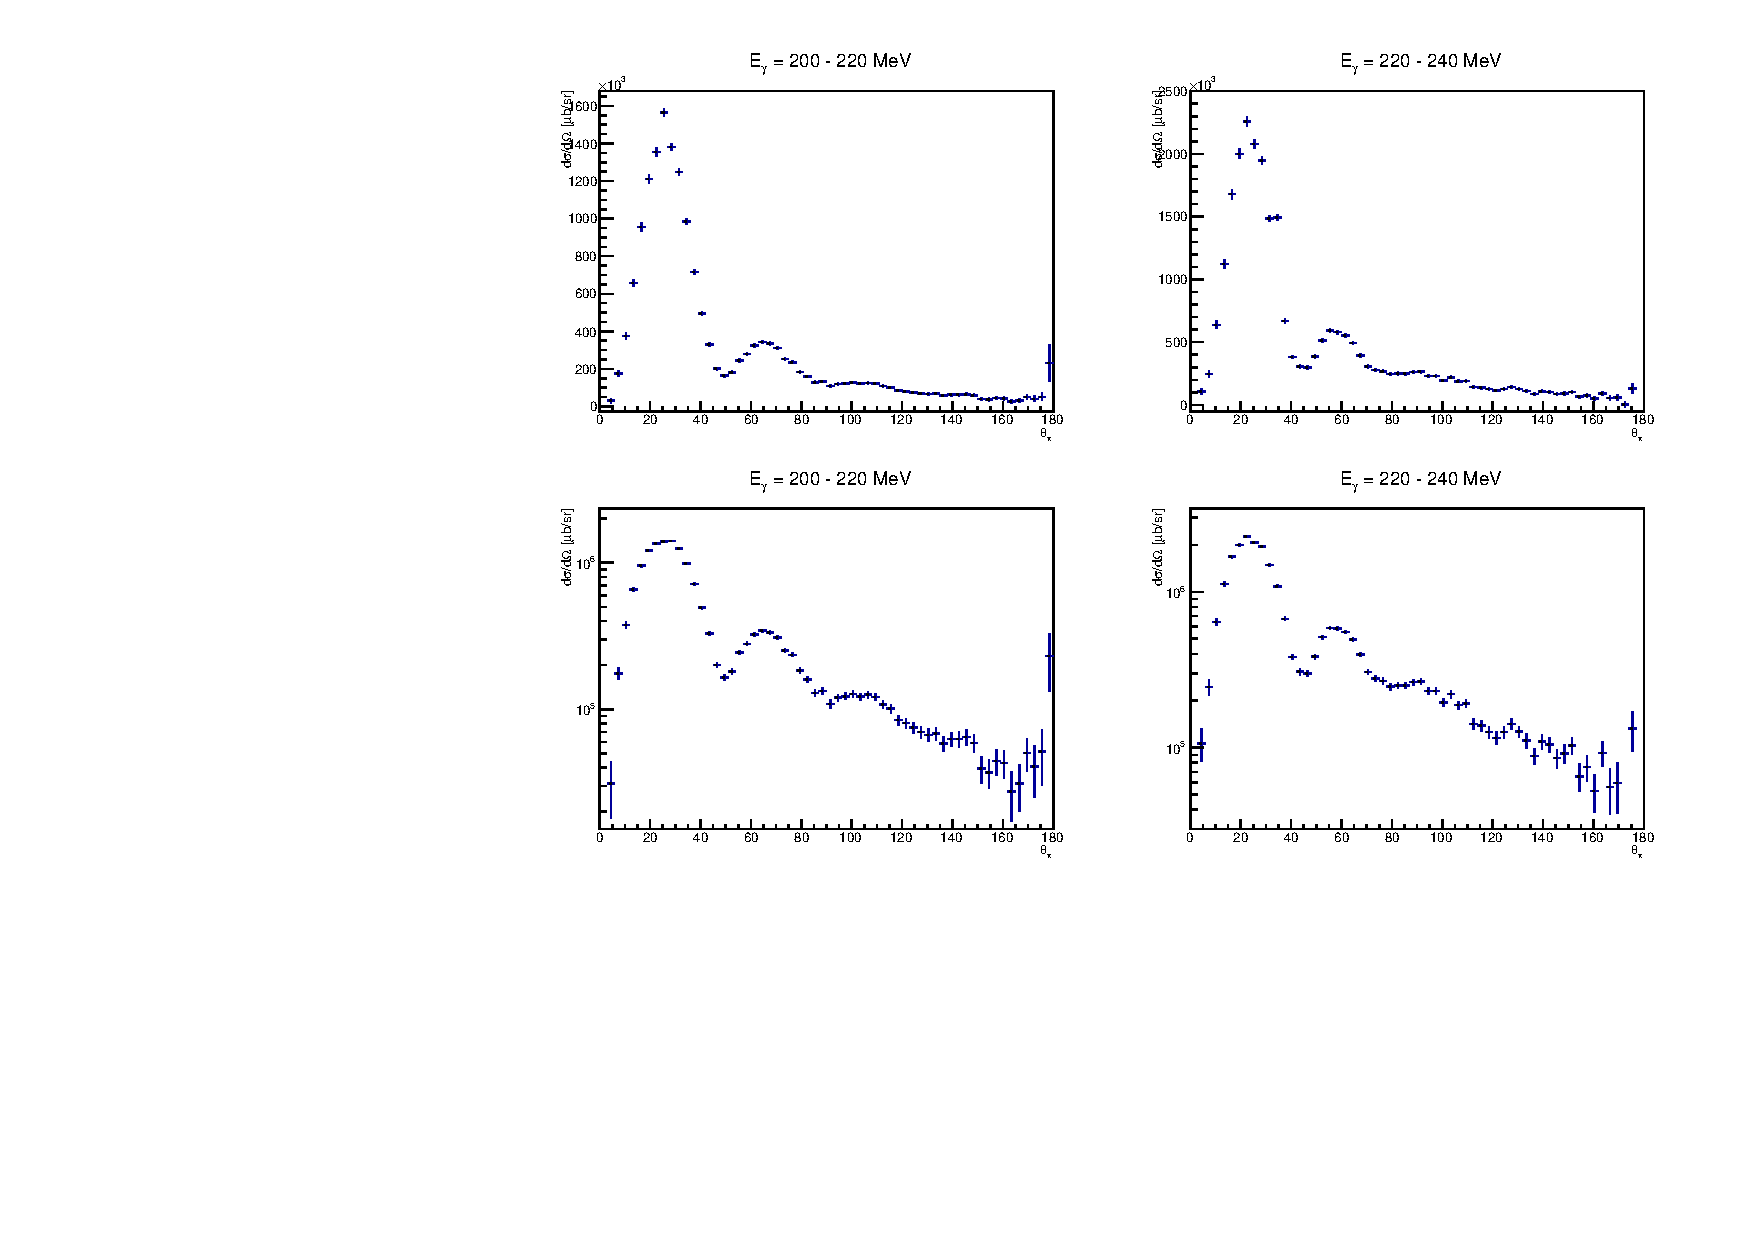
\includegraphics[scale=0.55]{pictures/pdf/sn116_cross_section_2.pdf}
\caption{Differential cross sections for the $^{116}Sn$ target for a sample of photon energy bins in the $E_{\gamma}$ range of $180 - 240 MeV$.}
\label{cross_section1}
\end{center}
\end{figure}
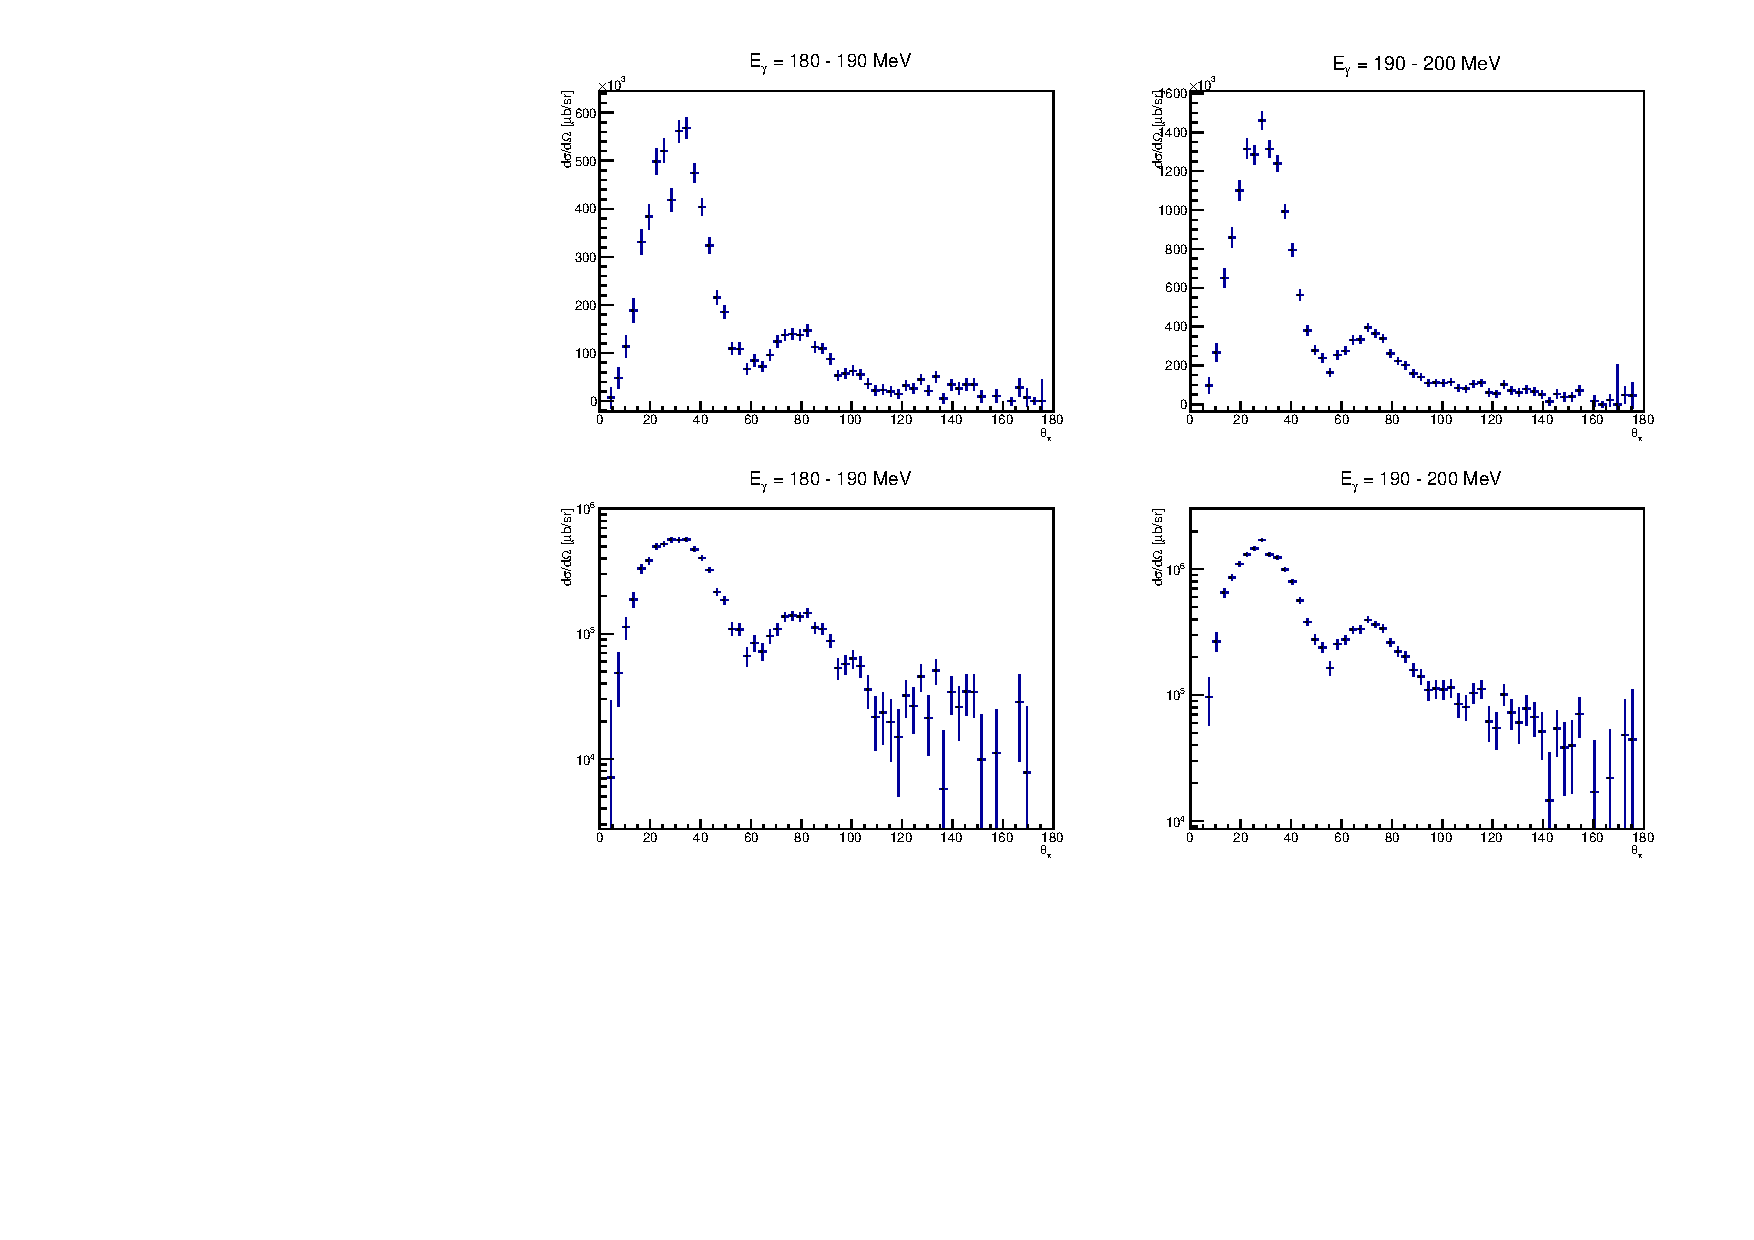
\includegraphics[scale=0.55]{pictures/pdf/sn120_cross_section_1.pdf}
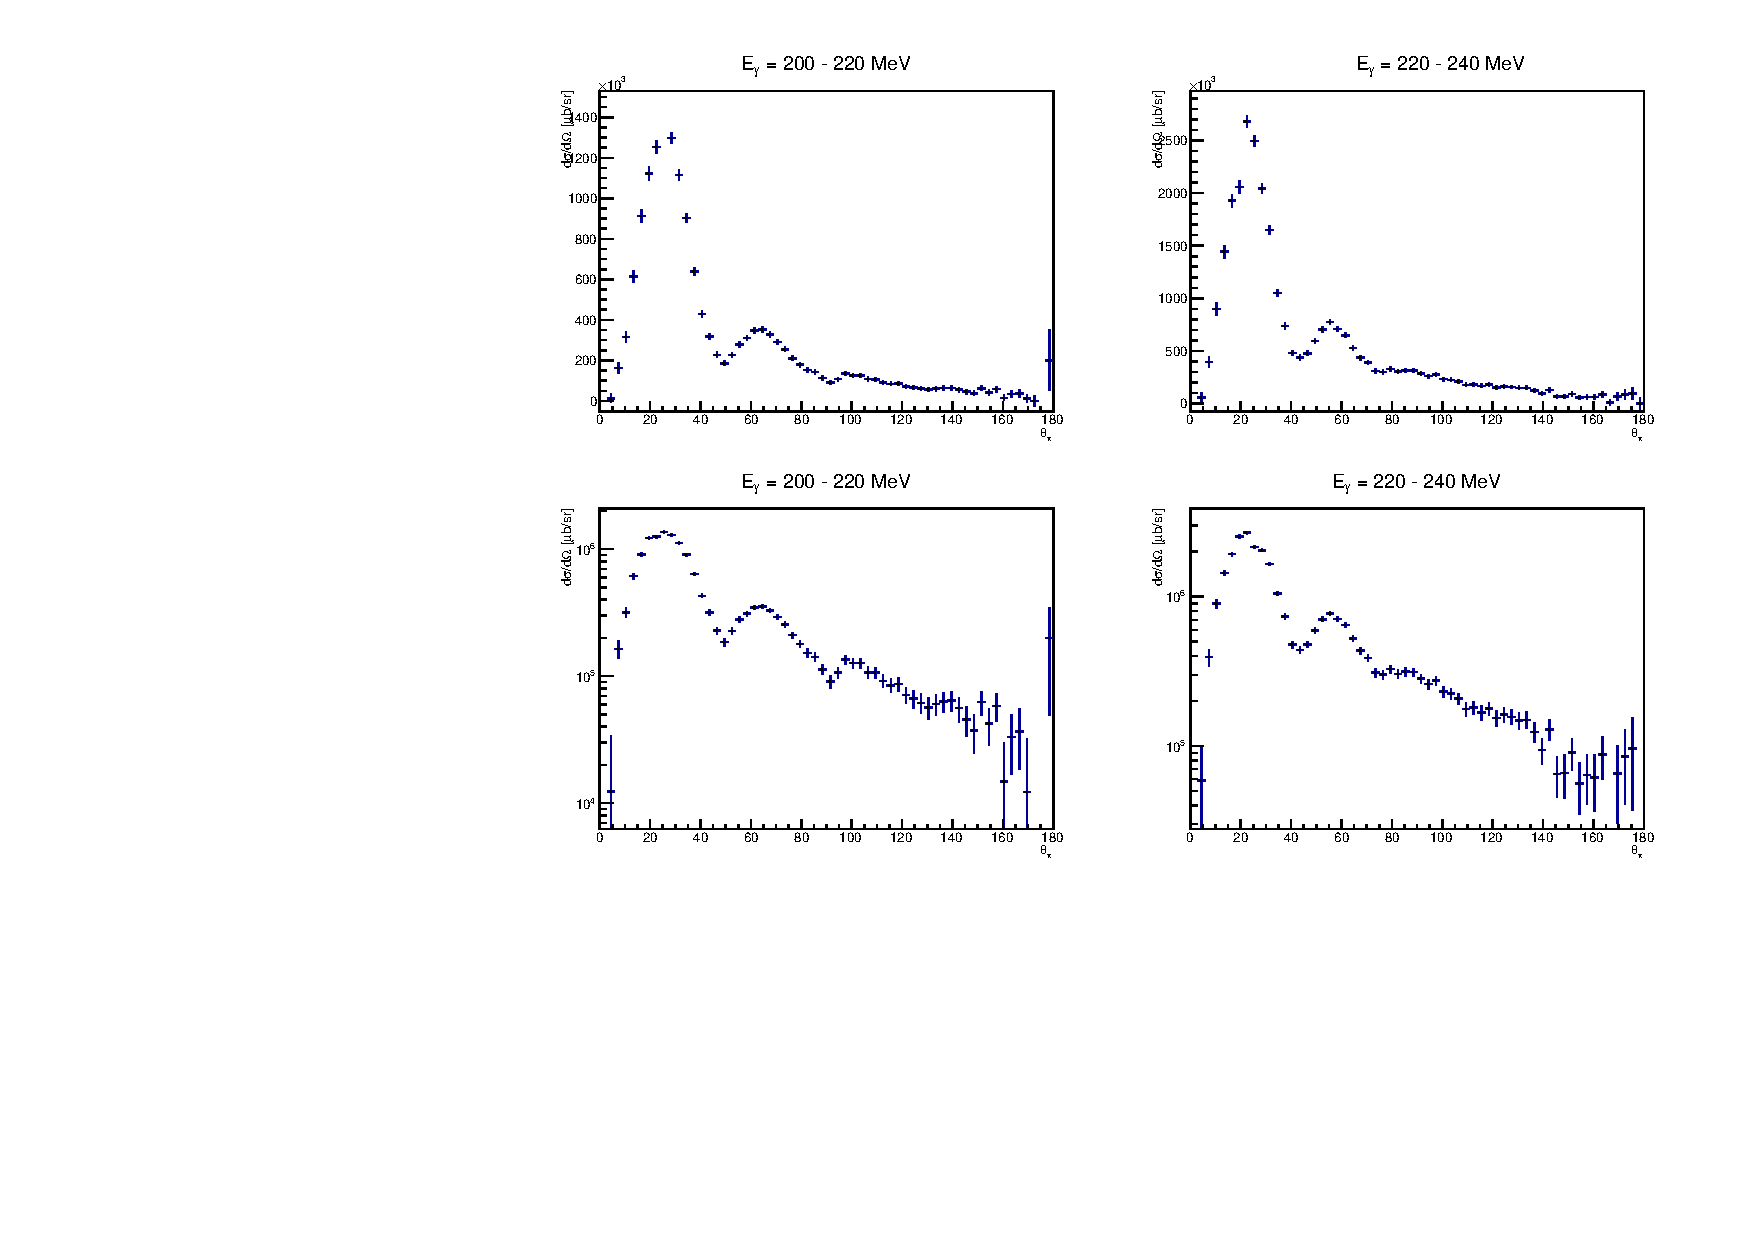
\includegraphics[scale=0.55]{pictures/pdf/sn120_cross_section_2.pdf}
\begin{figure}[H]
\begin{center}

\caption{Differential cross sections for the $^{120}Sn$ target for a sample of photon energy bins in the $E_{\gamma}$ range of $180 - 240 MeV$.}
\label{cross_section2}
\end{center}
\end{figure}

\begin{figure}[H]
\begin{center}
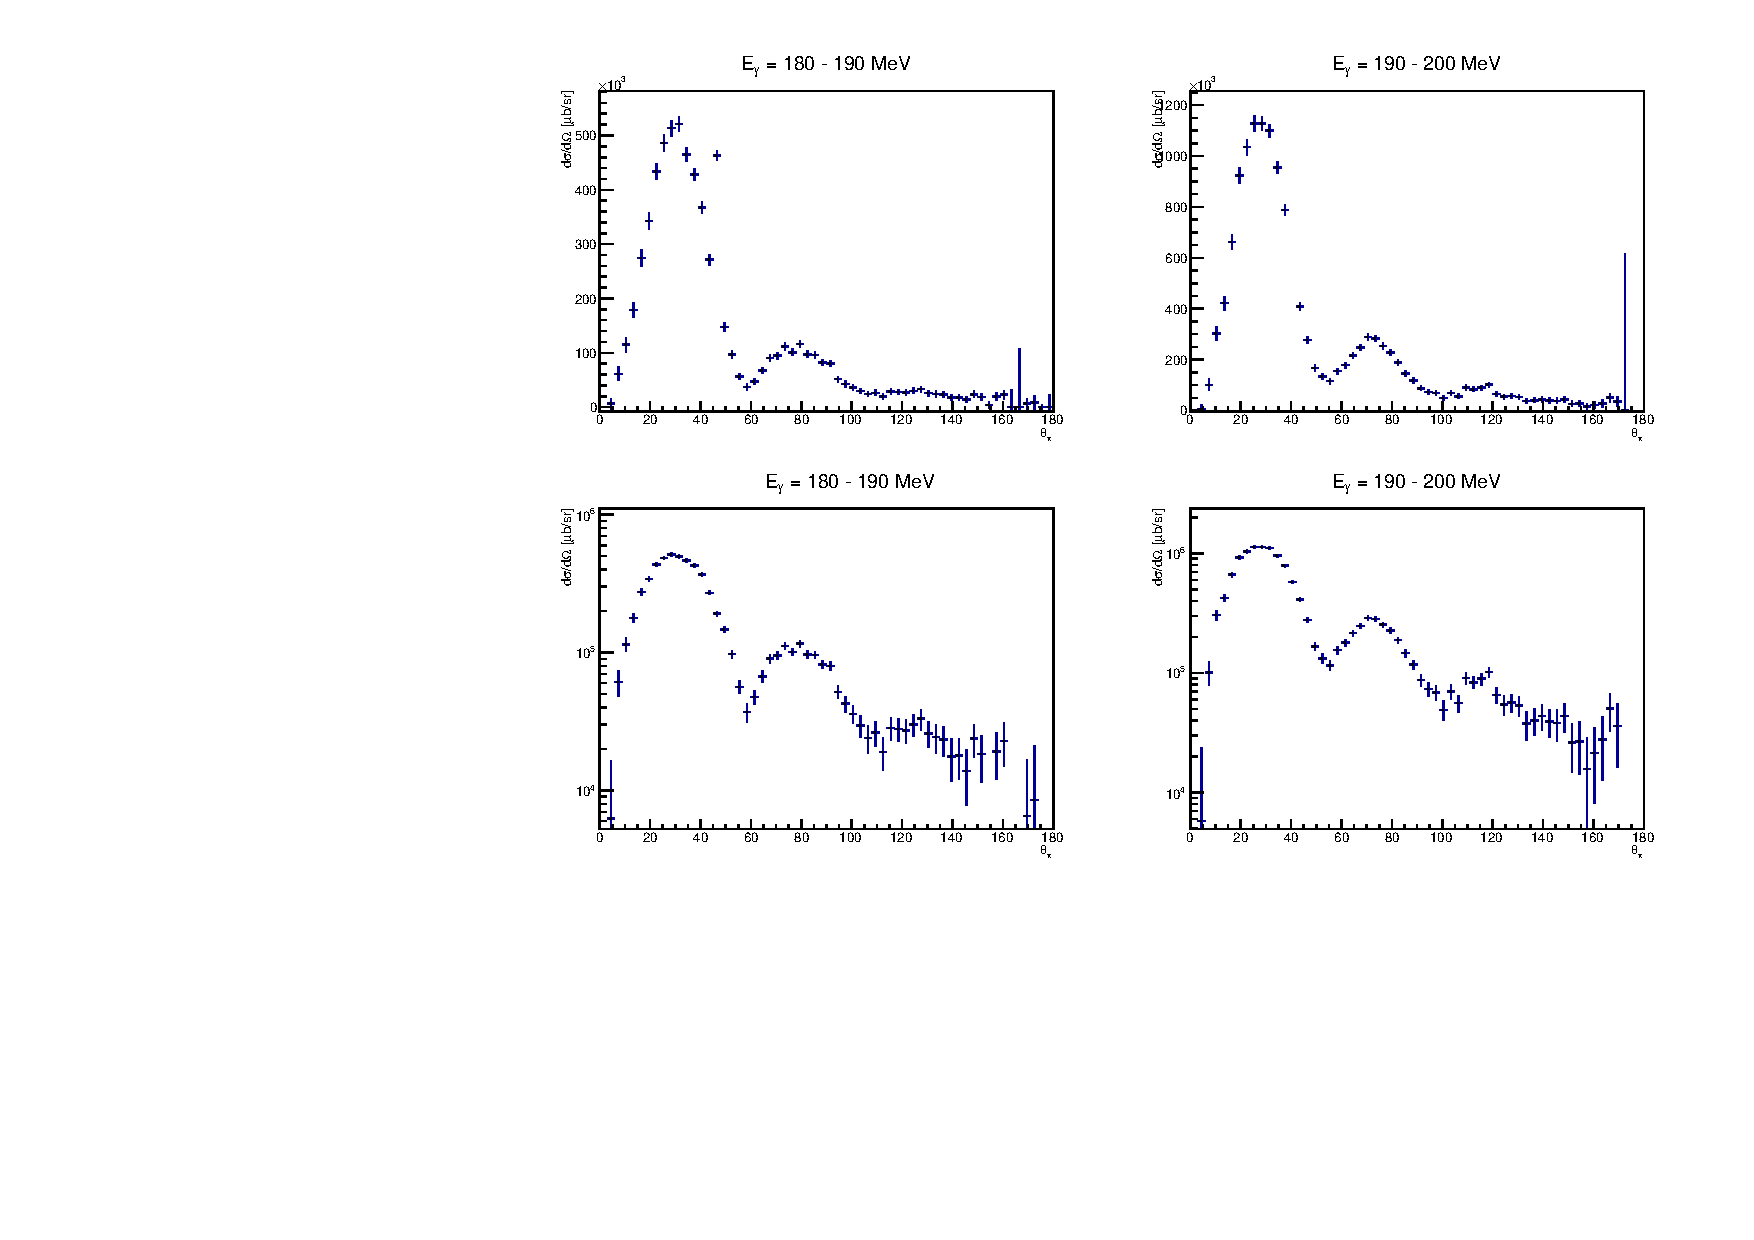
\includegraphics[scale=0.55]{pictures/pdf/sn124_cross_section_1.pdf}
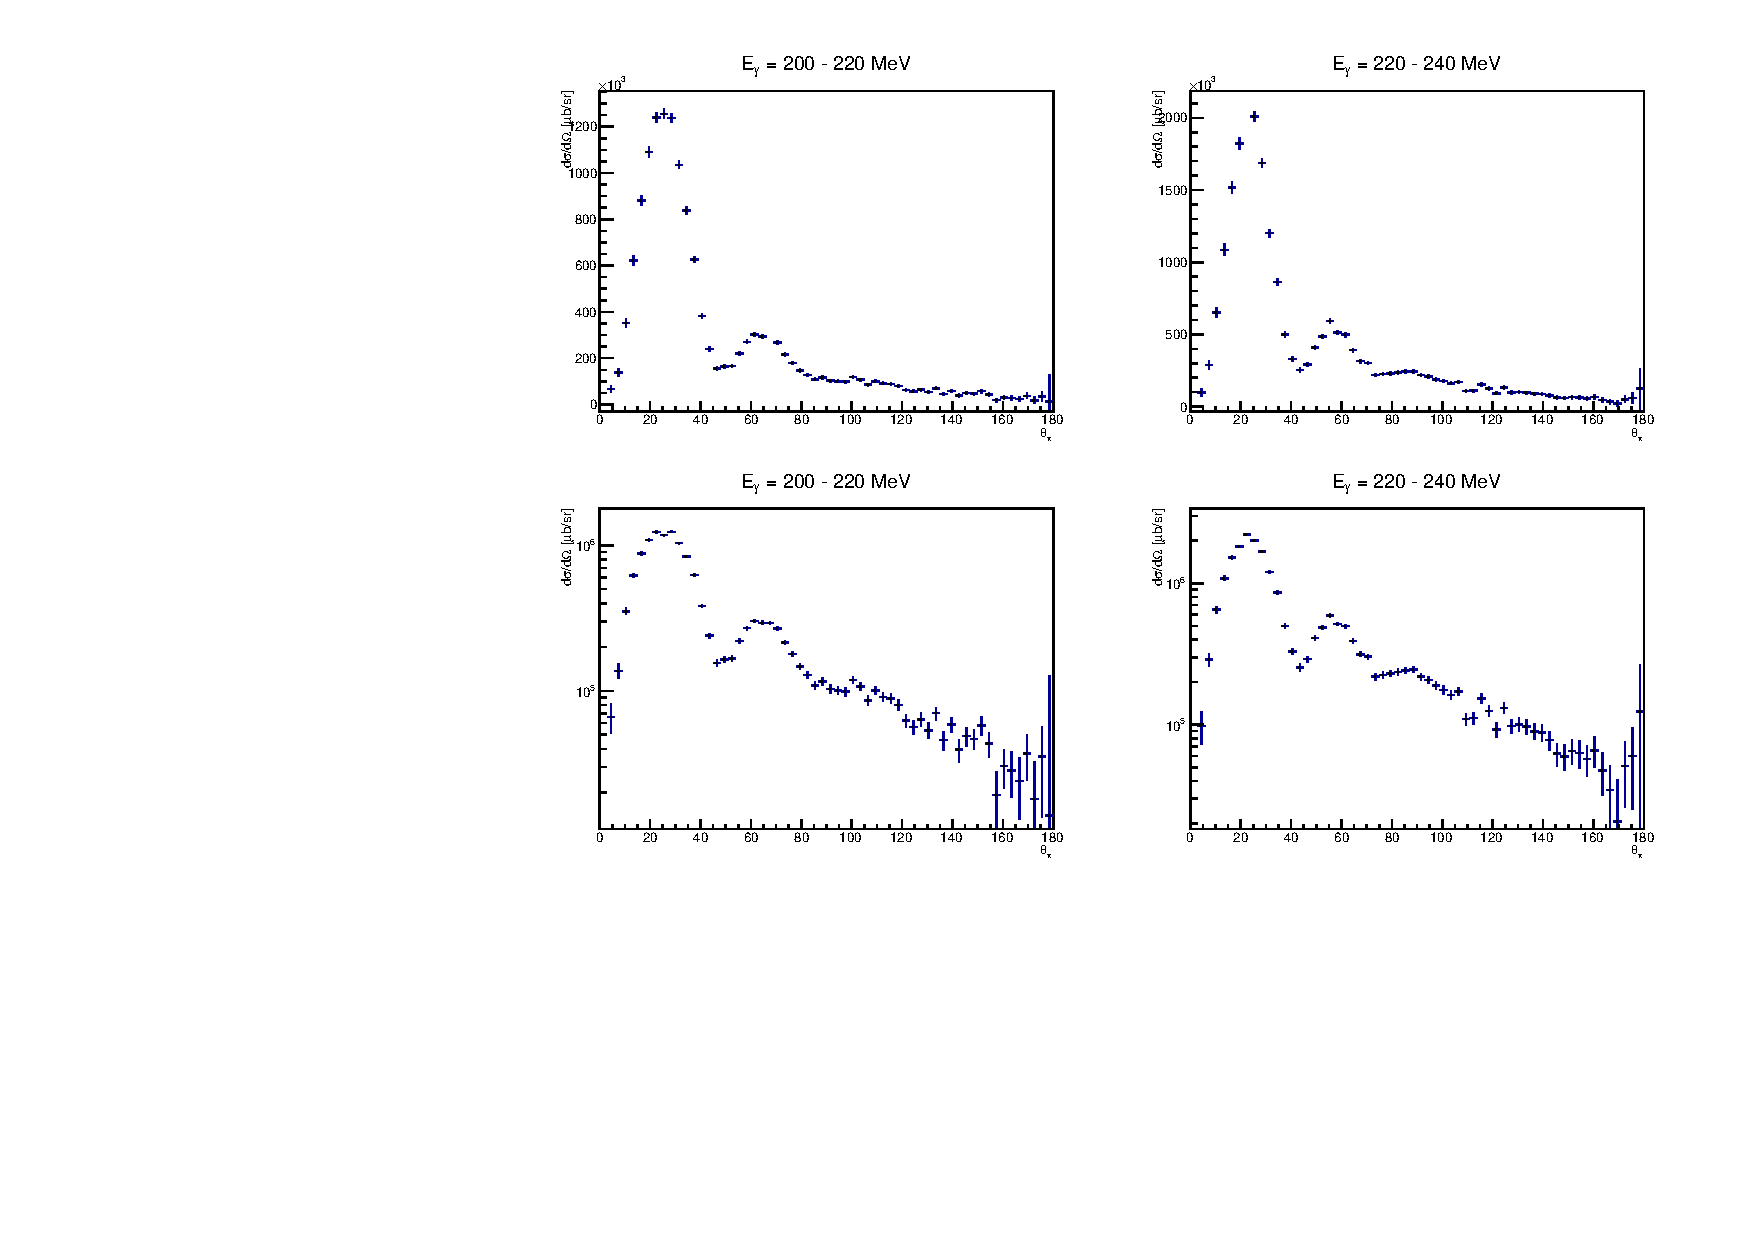
\includegraphics[scale=0.55]{pictures/pdf/sn124_cross_section_2.pdf}
\caption{Differential cross sections for the $^{124}Sn$ target for a sample of photon energy bins in the $E_{\gamma}$ range of $180 - 240 MeV$.}
\label{cross_section3}
\end{center}
\end{figure}

\indent The calculations of the ratio of cross sections have been performed in order to investigate the changes in the nuclear structure of the isotopes without the systematic error bias. Figures \ref{cross_ratio1} to \ref{cross_ratio3} present the ratios of the targets cross sections compared with the theoretical predictions from the Kamalov's DREN calculations, using the FSUGold parameter sets. The details of different FSUGold models are summarized in the Table \ref{fsu_table}.

\begin{figure}[H]
\begin{center}
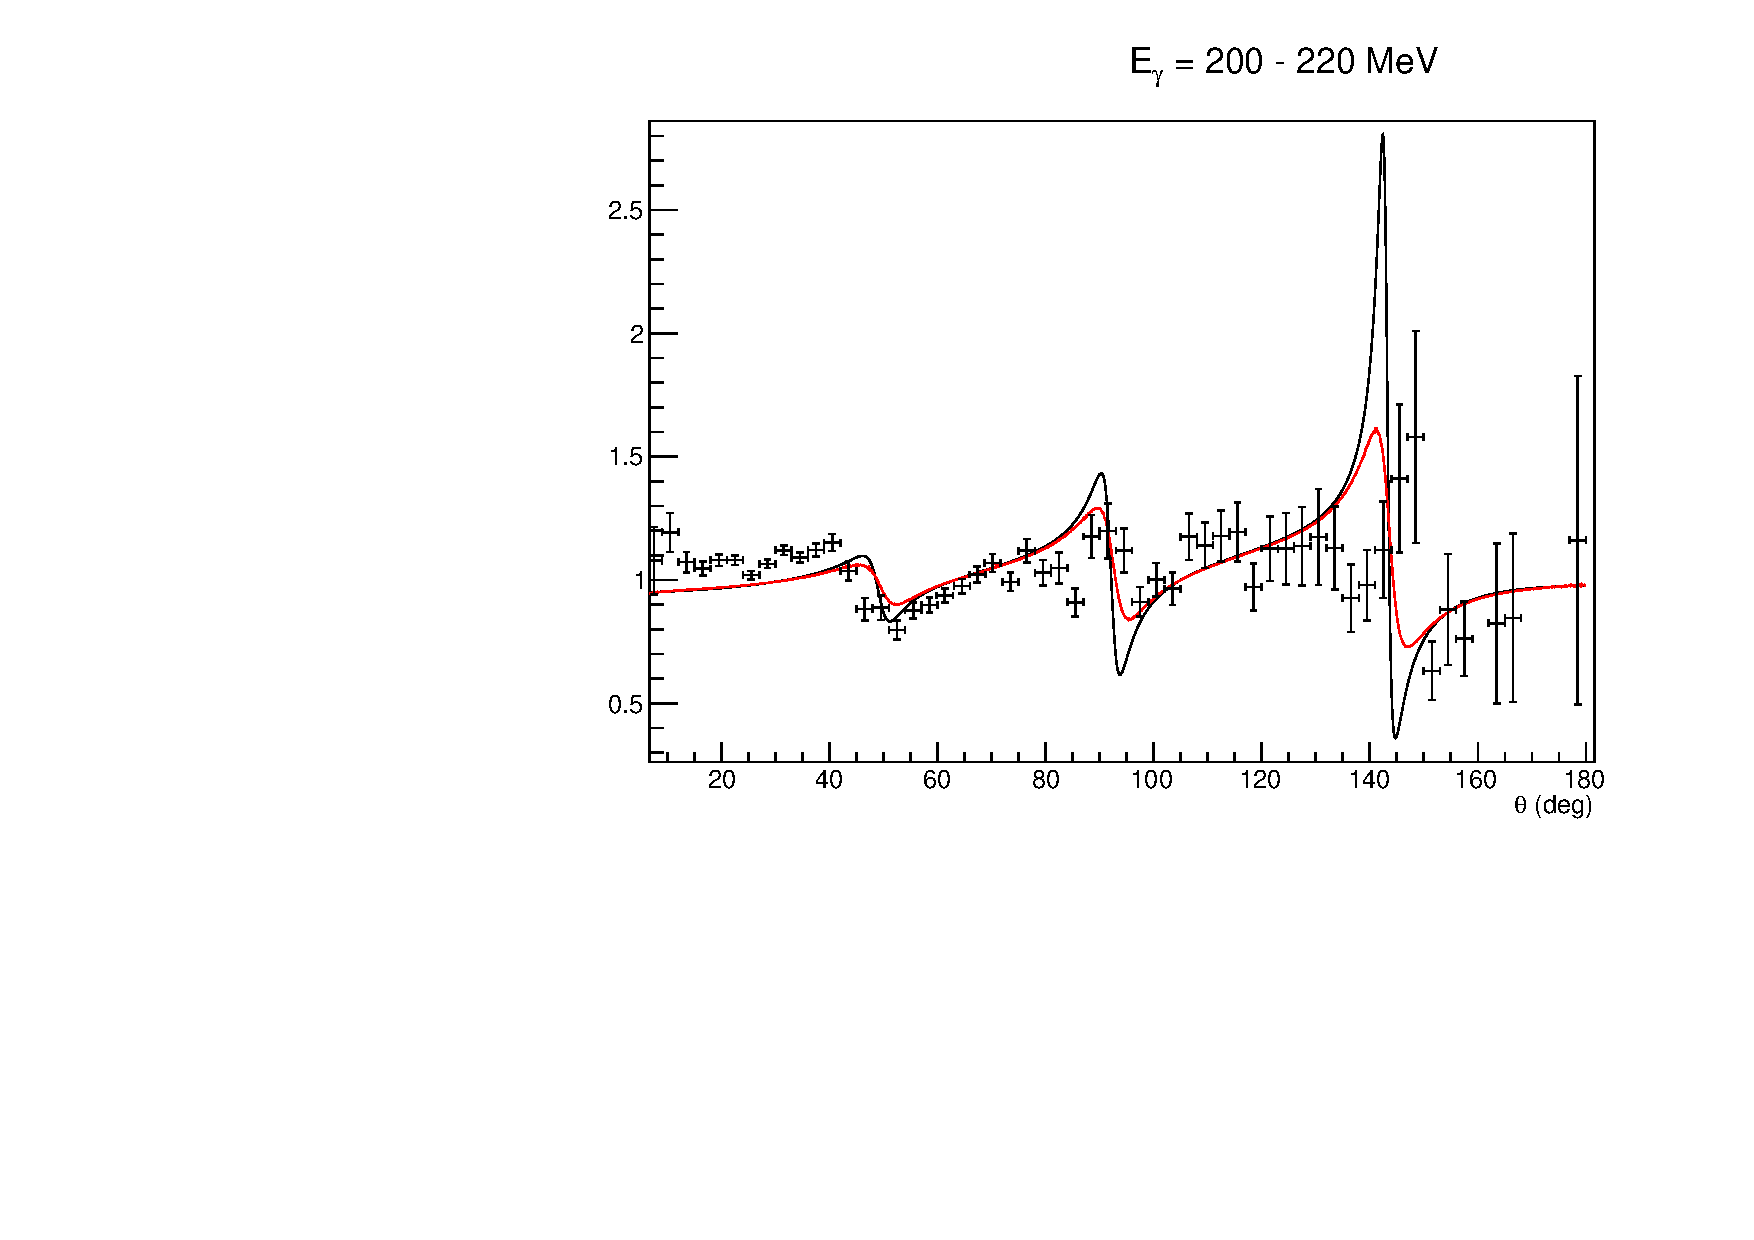
\includegraphics[scale=0.55]{pictures/pdf/cross_ratio_kamalov_Sn116_Sn120_Ebin8.pdf}
\caption{The ratio of the cross sections of $^{116}Sn$ to $^{120}Sn$ for the $E_{\gamma}$ bin $200 MeV$. The black line is the Kamalov's DREN calculations and the red line is those calculations smeared with the energy resolution.}
\label{cross_ratio1}
\end{center}
\end{figure}

\newcommand{\rastrech}[1]{\renewcommand{\arraystretch}{#1}}
\begin{table}[ht]
\rastrech{1.5}
\centering
\begin{tabular}{|c | c c c c c c c |}
\hline\hline
 & & &  FSU030 & & & &  \\
\hline
Isotope & $c_{p}$ (fm) &$b_{p}$ (fm) & $c_{n}$ (fm) & $b_{n}$ (fm) & $r_{p}$ (fm) & $r_{n}$ (fm) & $\Delta r$ (fm) \\
$^{116}Sn$ & 5.479 & 0.434 & 5.458 & 0.529 & 4.541 & 4.663  & 0.122\\
$^{120}Sn$ & 5.503 & 0.443 & 5.461 & 0.583 & 4.570 & 4.752  & 0.182\\
$^{124}Sn$ & 5.563 & 0.432 & 5.581 & 0.570 & 4.598 & 4.814  & 0.216\\
\hline\hline
 & & &  FSU010 & & &  &\\
\hline
Isotope & $c_{p}$ (fm) &$b_{p}$ (fm) & $c_{n}$ (fm) & $b_{n}$ (fm) & $r_{p}$ (fm) & $r_{n}$ (fm) & $\Delta r$ (fm) \\
$^{116}Sn$ & 5.464 & 0.435 & 5.484 & 0.531 & 4.530 & 4.685 & 0.155\\
$^{120}Sn$ & 5.482 & 0.444 & 5.496 & 0.585 & 4.556 & 4.780 & 0.224\\
$^{124}Sn$ & 5.541 & 0.433 & 5.622 & 0.572 & 4.584 & 4.846 & 0.262\\
\hline\hline
\end{tabular}
\caption{The FSUGold parameters set used for the Kamalov's DREN calculations. Two different values for the paramenters are used and compared with the data: FSU030 ....; FSU010 ....  Explaing the parameters briefly and recall it in the text where you will have a more detailed informations (Formulas, what they are, what their change inplies. 
!!!!IN CHAPTER 2 you say that you expect from the model a change in the isotopic chain of 0.05fm . From these values  you have 0.094 and 0.107. Change chapter 2 and have a label to here from there and viceversa. By the way, put the units!!! }
\label{fsu_table}
\end{table} 

\indent The dependence of the energy resolution on $\theta$ for different targets and photon energies is shown in the figures below. Those data have been fitted with a third degree polynomial function wich was then used in the DREN calculations to reflect the effect of the energy resolution on the ratio of the cross sections predictions.

\begin{figure}[H]
\begin{center}
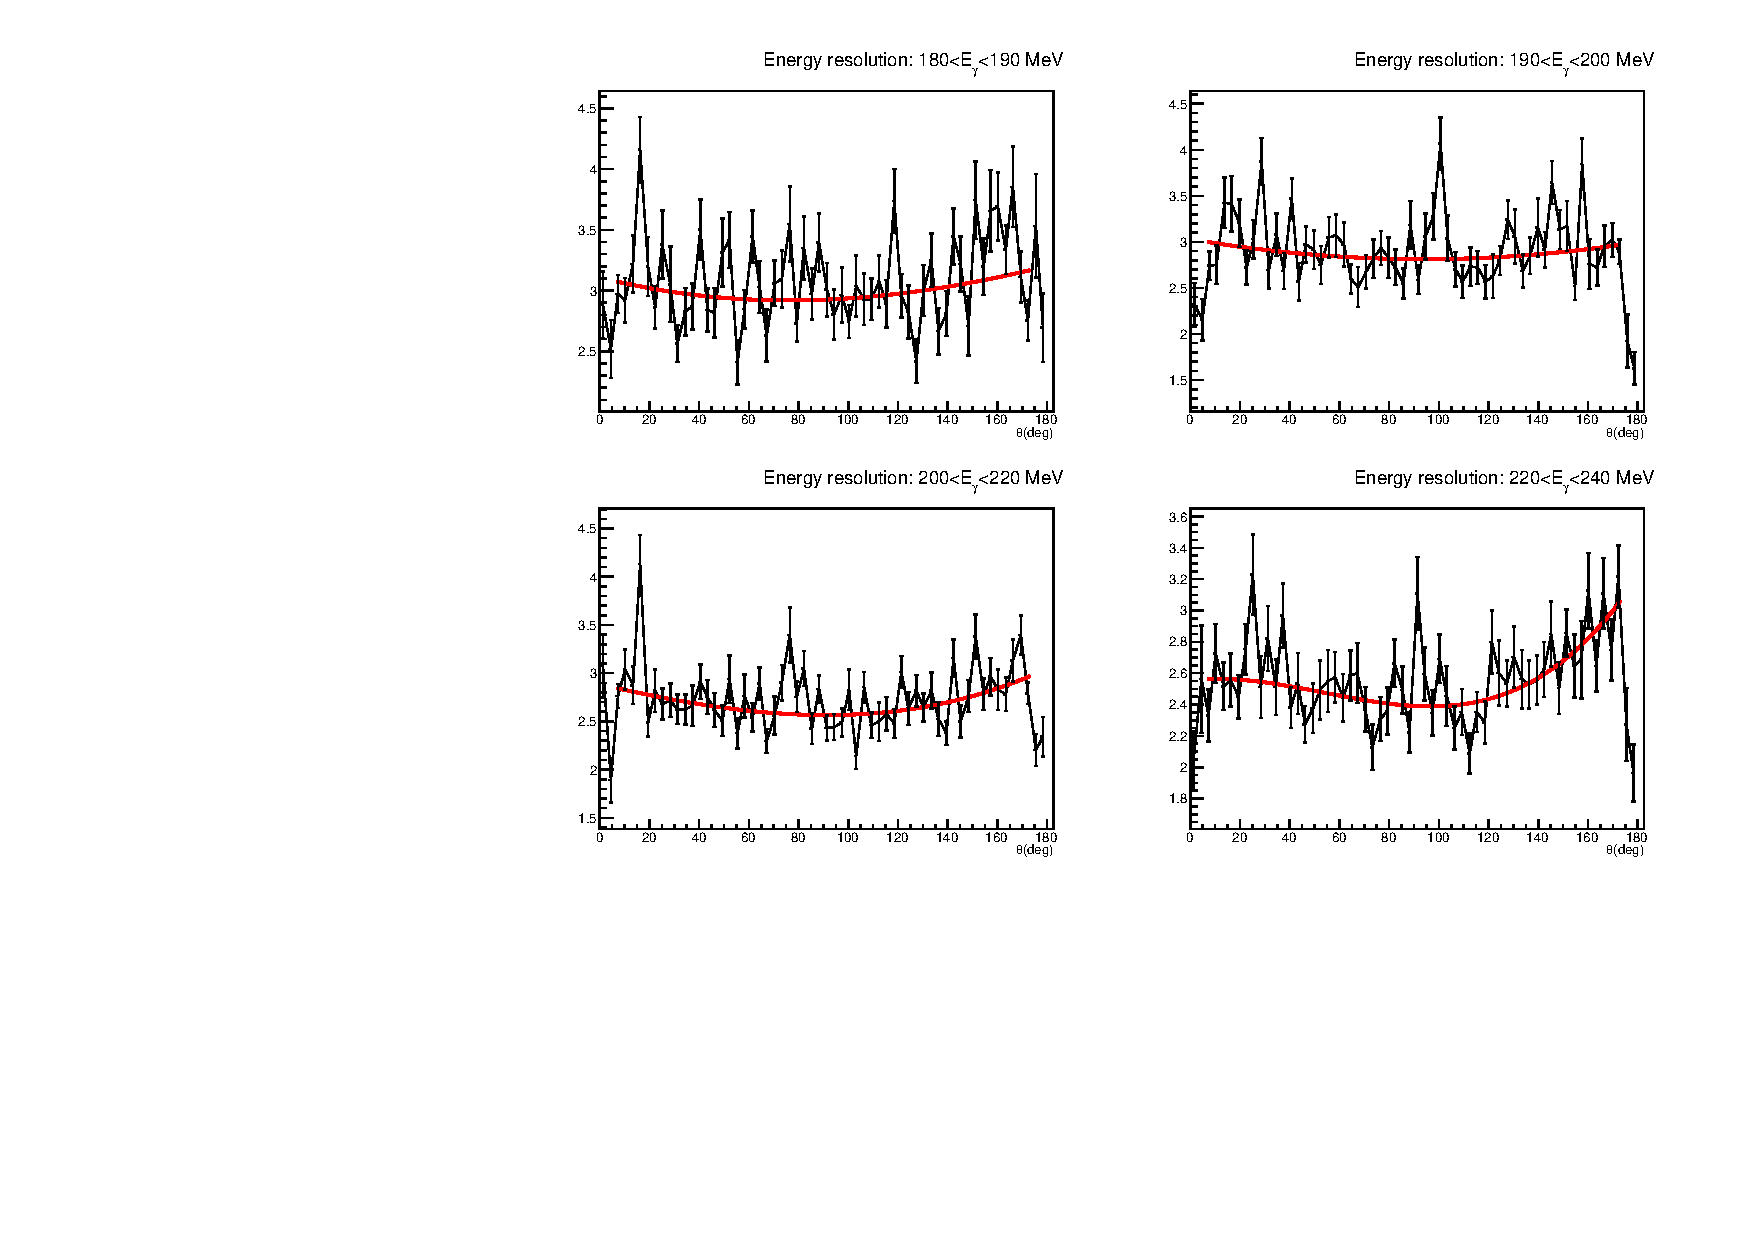
\includegraphics[scale=0.75]{pictures/pdf/energy_resolution_sn116.pdf}
\caption{Plots of the energy resolution dependence on $\theta$ and $E_{\gamma}$ for the $^{116}Sn$ target.}
\label{energy_res1}
\end{center}
\end{figure}